\documentclass{article}

\usepackage{fancyhdr}
\usepackage{mathtools}
\usepackage{amsmath}
\usepackage{amssymb}
\usepackage{amsfonts}

\pagestyle{fancy}

\author{
  Robin Touche \\
  \and
  Fredrik Bredmar
}

\title{Machine Learning Homework 5}

\begin{document}

\maketitle

\subsection*{1.1}

\subsection*{1.2}
\paragraph{a}

We wish to find a solution to

\begin{align}
  arg \min_{(\mathbf{w}, b)} \frac{1}{2} \lvert \rvert \mathbf{w}^2 \lvert \rvert
\end{align}
subject to the constraint that for all $i = 1, ... , n$

\begin{align}
  y_i (\mathbf{w} \cdot x_i - b) \geq 1
\end{align}
Using the Lagrange multiplier method this can be expressed as

\begin{align}
  arg \min_{(\mathbf{w}, b)} \max_{a > 0} \left\{ \frac{1}{2} \lvert \rvert \mathbf{w}^2 \lvert \rvert -
      \sum_{i = 1}^{n}\alpha_i \big( y_i \left( \mathbf{w} \cdot x_i - b \right) - 1 \big) \right\}
\end{align}
Which can be simplified to

\begin{align}
  \mathbf{w} = \sum_{i = 1}^{n}\alpha_i y_i x_i
\end{align}

%TODO derive

\begin{align}
  b = \frac{1}{N_{SV}} \sum_{i = 1}^{N_{SV}} \left( \mathbf{w} \cdot x_i - y_i \right)
\end{align}

\paragraph{b}

\subsection*{2.1}
\paragraph{a}
See code.

\paragraph{b}
The support vectors are marked as filled points. \\
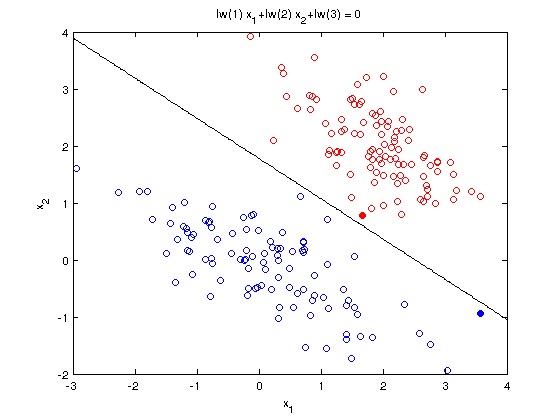
\includegraphics[scale = 0.7]{pics/plot21.png}

\paragraph{c}
It has a bias of $\approx 1.7785$.

\paragraph{d}
The margin $\gamma$ is $\approx 0.1523$.

\subsection*{2.2}
\paragraph{a}
The filled points are corretly classified.\\
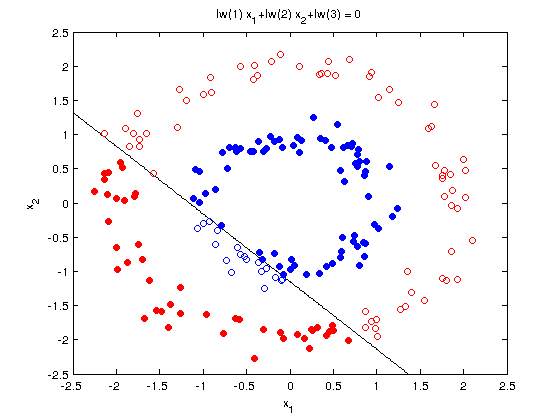
\includegraphics[scale = 0.7]{pics/plot22.png}

\paragraph{b}

Using SMO:

\begin{tabular}{c | c | c}
  Kernel & Execution time ($s$)& CV accuracy\\
  \hline
  Linear & 0.0236 & 51\%\\
  Quadratic & 0.0177 & 100\%\\
  RBF & 0.0104 & 100\%
\end{tabular}\\

Using QP:

\begin{tabular}{c | c | c}
  Kernel & Execution time ($s$)& CV accuracy\\
  \hline
  Linear & 0.0080 & 51\%\\
  Quadratic & 0.4746 & 100\%\\
  RBF & 0.3152 & 100\%
\end{tabular}

\end{document}
